\documentclass{article}

\usepackage[english]{babel}
\usepackage[utf8x]{inputenc}
\usepackage{amsmath}
\usepackage{graphicx}
\usepackage[colorinlistoftodos]{todonotes}
\usepackage{fullpage}
\usepackage[letterpaper,
top    = 1.25in,
bottom = 1in,
left   = 1.25in,
right  = 1.25in]{geometry}
\usepackage{indentfirst}
\usepackage{enumitem}

\title{\Huge{\textsf{Budgetory} \\ Final Report \\ \vspace{35px} \Large{Team 15}}}
\author{
Bruce, Daniel\\
\texttt{bruced@rpi.edu}
\and
Cheung, Sammi\\
\texttt{cheuns2@rpi.edu}
\and
Sedlacek, Aaron\\
\texttt{sedlaa@rpi.edu}
}

\date{\vfill{} \large{December 5, 2013}}

\begin{document}
\begin{center}
\Large{\textsc{Rensselaer Polytechnic Institute} \\ Introduction to Information Technology and Web Science}
\end{center}
{\let\newpage\relax\maketitle}
\thispagestyle{empty}
\newpage


\section{Description}
\textsf{Budgetory} is a full-featured, web-based budgeting and inventory application designed for organizations dealing with those items. \textsf{Budgetory} allows for sharing and collaboration between multiple users, all of whom can control multiple budgetories. In addition, the owner of a budgetory can control permissions for each linked user. 


\vspace{40pt}

\section{Who \textsf{Budgetory} serves}
\vspace{20px}
\subsection{Social organizations}
Being at RPI, our main target for \textsf{Budgetory} is fraternities and sororities. Greek life organizaions deal with oftentimes large budgets over the course of a semester. Additionally, most chapters---organizationally-modeled after and run as a house---keep many different supplies on hand---from food to bathroom tissue, mop heads to sponges. 

We also cater to other social organizations, like Veterans of Foreign Wars posts.
\vspace{20px}
\subsection{Service organizations}
Another cohort of groups \textsf{Budgetory} suits is service organizations. While they may not deal with the extensive, constantly changing inventory of fraternity-like associations, their budgets can be very active.

Groups like Lions Clubs International, Kiwanis International, and Rotary International fundraise throughout the fiscal year, hold large service events and give scholarships, and have to track their finances constantly. Our application provides easy access to all of their important information.

\vspace{40pt}
\section{\textsf{Budgetory} in the context of existing applications}\label{crossone}
\textsf{Budgetory} falls in the middle of the oft-used database application realm. It combines the best of both worlds---financial software and inventory tracking---and adds features not included in either.

Many different solutions exist for financing and inventorying individually, but not both together. Software packages like \emph{Quickbooks} and \emph{Quicken} can be very useful and helpful keeping track of money. \emph{Microsoft Excel} works well for bookkeeping, also, but can take time to set up. Lastly, \emph{Microsoft Access} can handle both budgets and inventories, but has a very steep learning curve and takes an enormous amount of time to prototype, build, and implement.

No existing products that we know of give users an easy way to share their statistics, the only exception being Mint. Mint, by Intuit, is web-based, so, theoretically, one could give credentials to another person. That being said, permissions cannot be managed by the owner, and data cannot be shared; only a user's credentials can be---something which is not secure.

For years, the only method of tracking funds and product stock was using paper and pencil. This is not secure---neither in a financially sensitive nor a loss prevention way. If the notebook tracking data was damaged, lost, or stolen, all data would be lost.

\vspace{40pt}
\section{\textsf{Budgetory}'s value}
\vspace{20pt}
\subsection{How \textsf{Budgetory} distinguises itself}
As stated above, \textsf{Budgetory} fills a void in the tracking software world. There is currently no shareable, permission-modifiable, web-based, non-bespoke application on the market. \textsf{Budgetory} provides these features in a lightweight package, accessible from anywhere one has an internet connection.

\vspace{20pt}
\subsection{Demand for \textsf{Budgetory}}
Through an unscientific survey, we found that the demand for a new method---most organizations are using  methods listed in section \ref{crossone}---of financial and inventory tracking is quite high. Most respondents listed their current method satisfaction as "I manage," which was in the middle of a five-level scale. We also polled factors influencing purchase, in which organization and efficiency were listed as the most desirable. Being web-based and lightweight, \textsf{Budgetory} provides those characteristics.

\vspace{40pt}
\section{Information architecture}
\textsf{Budgetory} was built to be lightweight and easily deployable on AMP stacks. It incorporates PHP scripting to access a MySQL database.

\vspace{20pt}
\subsection{Platform}
Although developed using Apache via XAMPP, any PHP-capable web server can run the code for \textsf{Budgetory}.

\vspace{20pt}
\subsection{Database}
\textsf{Budgetory} uses a MySQL database. On new deployments, a database initialization file is used to create the correct framework.
{\centering 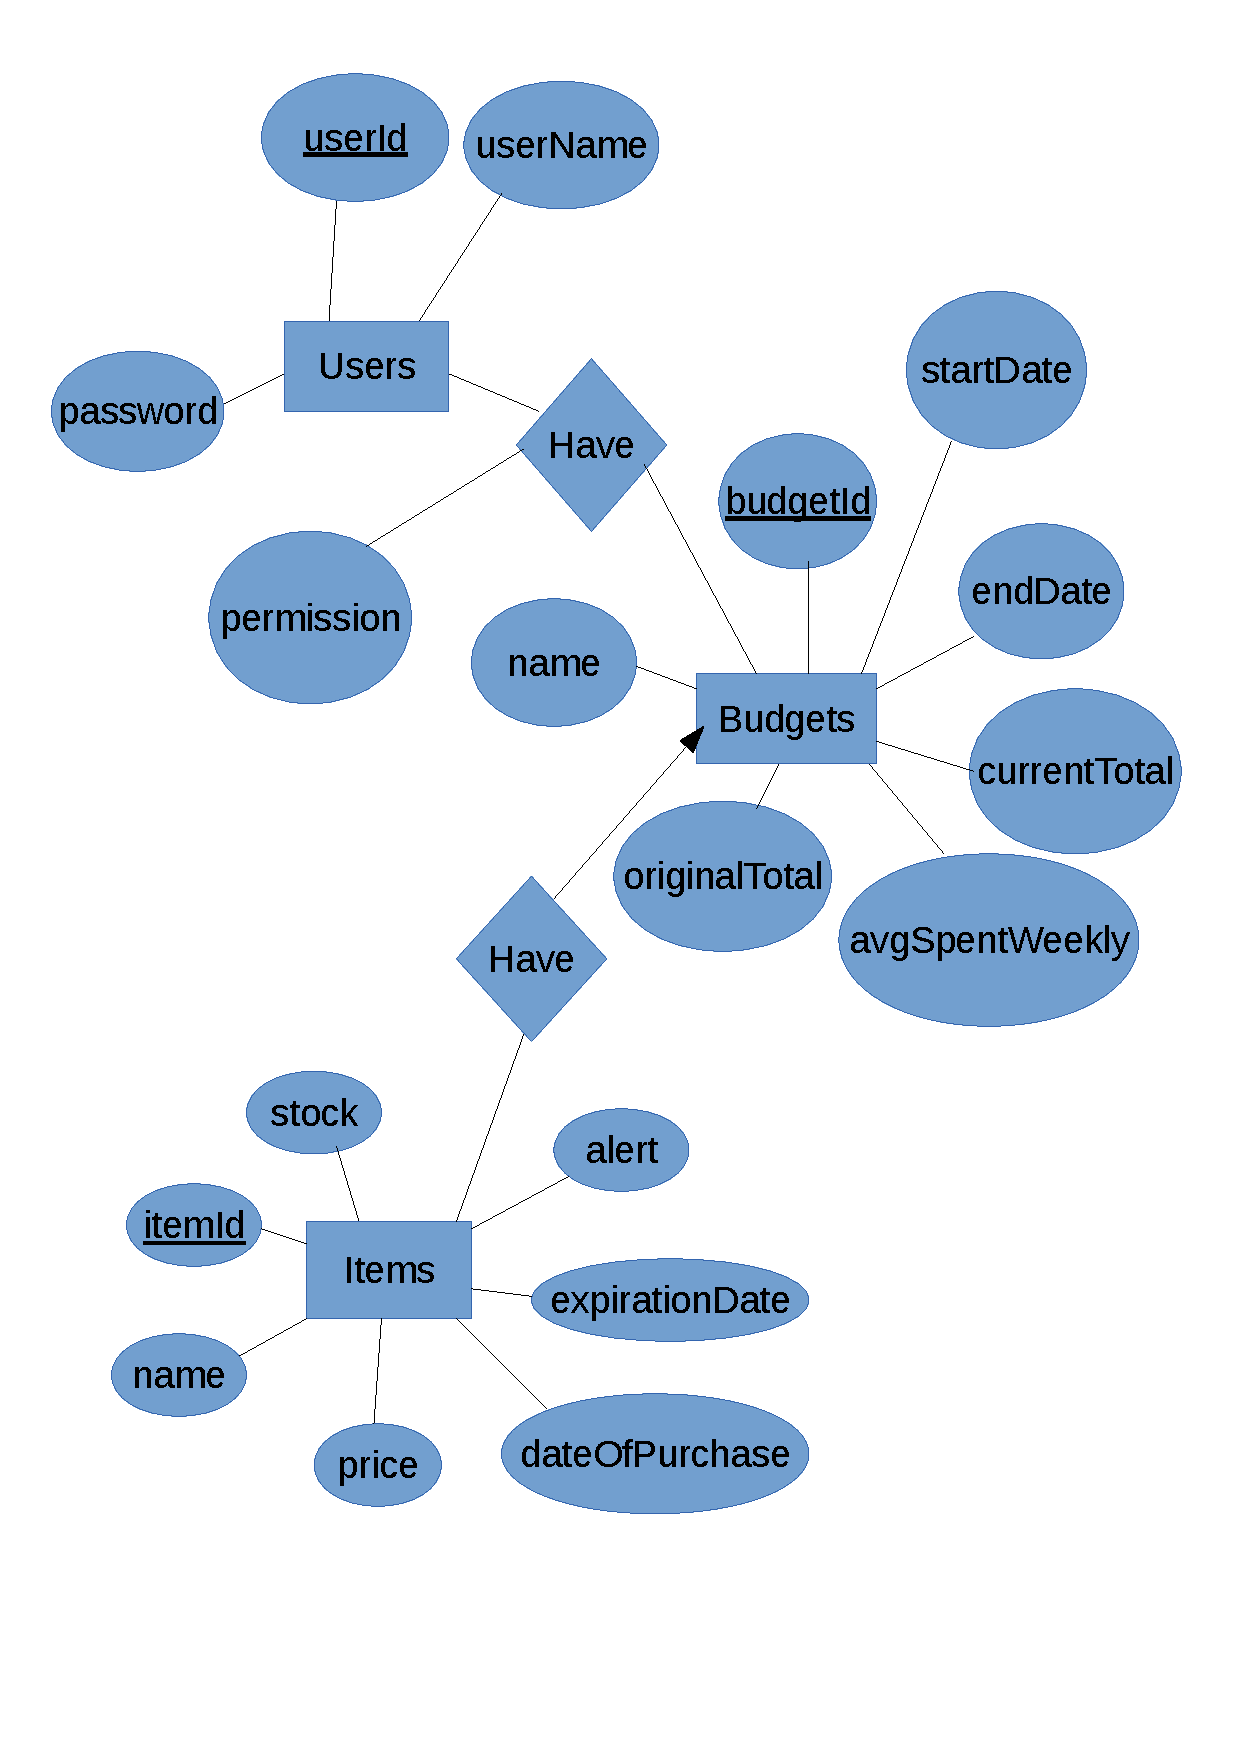
\includegraphics[width=3.5in,page=1,keepaspectratio]{ER_diagram_graphic.pdf} \par}

User information is stored in \texttt{Users}. Attributes stored include \texttt{userID} (the primary key), \texttt{userName}, and \texttt{password} (which is both salted and hashed using bcrypt).

Budget and inventory information is stored in \texttt{Budgets} and \texttt{Items}, respectively.

\texttt{Budgets} includes the attributes \texttt{budgetId} (the primary key), \texttt{name}, \texttt{startDate}, \texttt{endDate}, \texttt{currentTotal}, \texttt{avgSpentWeekly}, and \texttt{originalTotal}.

\texttt{Items} includes the attributes \texttt{itemId} (the primary key), \texttt{name}, \texttt{price}, \texttt{dateOfPurchase}, \texttt{expirationDate}, \texttt{stock}, and \texttt{alert}.

Relationships between tables are as follows:
\begin{itemize}[noitemsep, nolistsep]
\item Users can have multiple users
\item Budgets can have multiple users
\item Budgets can have multiple budgets
\end{itemize}

User--budget relationships are managed and stored in a mapping table, \texttt{userToBudget}. \texttt{userToBudget} also stores an attribute called \texttt{permission}, which stores a \texttt{1}, \texttt{2}, or \texttt{3} value for each user--budget relationship.

\vspace{20pt}
\subsection{Database access}
Reading and writing to the database is performed using PHP. Before any function is performed, a session-checking function is called. This function, called \texttt{userCheck}, checks a cookie for the time of the last performed function. If it has been more than a specified length of time, the user has effectively timed-out, and they are forced to log back in. For security, whatever manipulation they attempted to perform immediately before getting denied access is not initiated.

If a user exits their browser, upon return, they will be forced to log back in---even if the specified timeout period has not fully elapsed. If a user exits a tab or navigates to another website but  returns within the specified timeout period, they will be allowed to continue working. This is implemented using a PHP session specific to the user.

\vspace{40pt}
\section{Future plans}
Future plans for \textsf{Budgetory} include:
\begin{itemize}
\item Mobile-styled website
\item Native mobile application
\item HTTPS security
\item Email and SMS alerts for settable budgetory conditions
\end{itemize}


\end{document}